\section{Package Server}
In questa sezione verranno descritti il package \texttt{server} e le classi che lo compongono.\\

\begin{figure}[H]
    \centering
    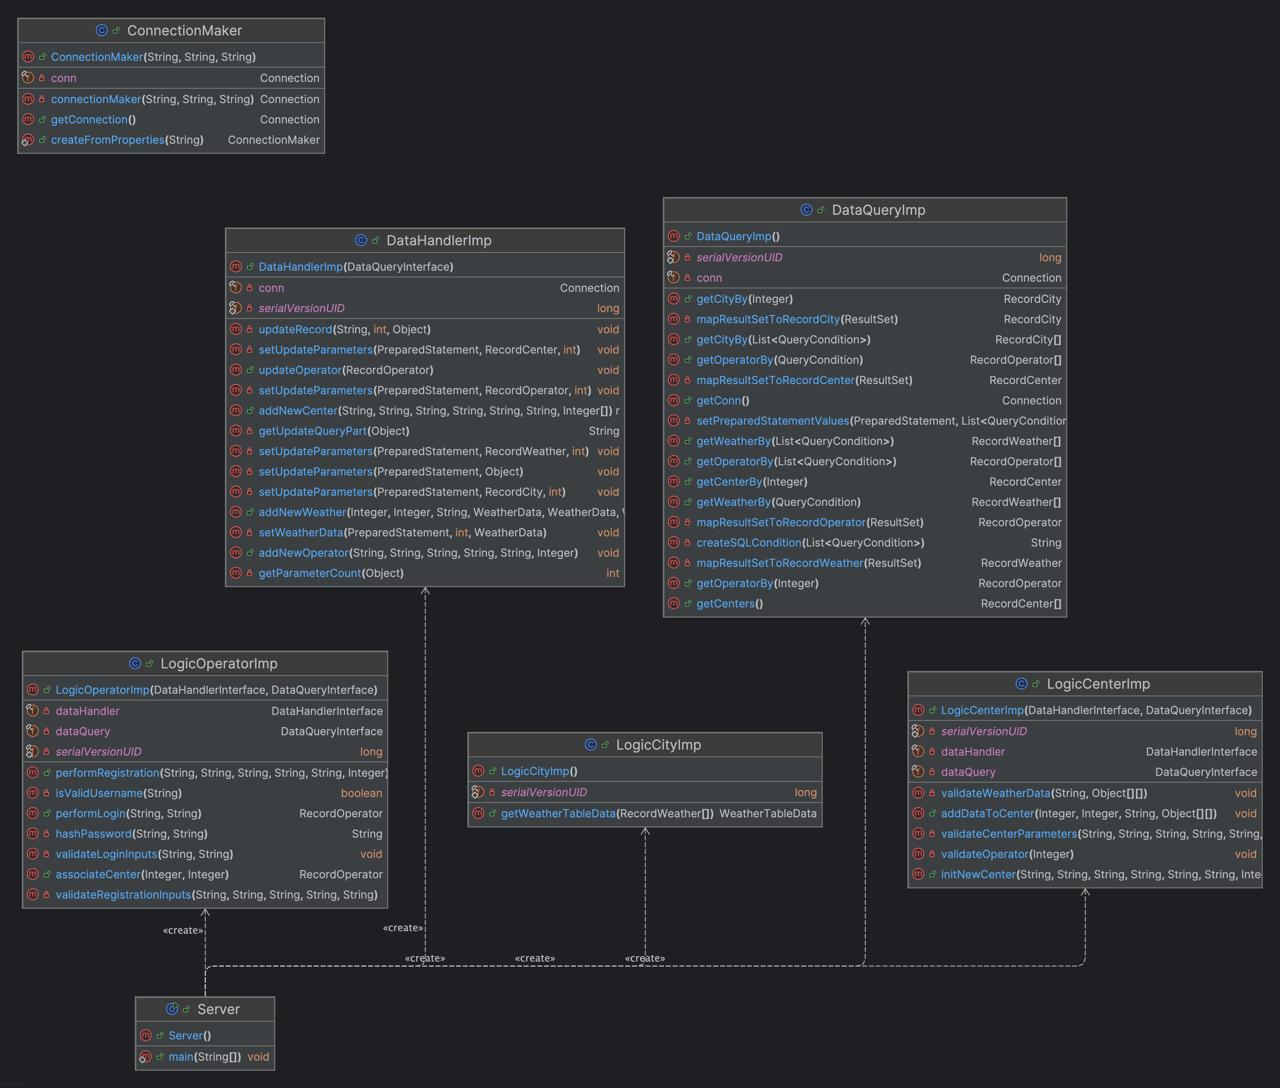
\includegraphics[width=0.9\textwidth]{img/serverClassDiagram.jpg}
    \caption{UML del package Server}
    \label{fig:Server}
\end{figure}

\subsection{Server}
La classe \texttt{Server} è progettata per avviare il registro RMI e pubblicare le implementazioni delle interfacce remote.\\
Queste implementazioni sono accessibili ai client remoti, che possoo invocare metodi per interrogare, gestire e manipolare i dati relativi alle operazioni dell'applicazione.\\
In sisntesi, \texttt{Server} svolge le seguenti operazioni principali:
\begin{itemize}
    \item \textbf{Creazione e Configurazione del Registro RMI}: avvia un registro RMI sulla porta specificata (di default, la porta 1099) utilizzando il metodo\\
          \texttt{LocateRegistry.createRegistry(int port)}. Questo registro permette ai client remoti di trovare e invocare i metodi delle interfacce registrate.
    \item \textbf{Inizializzazione delle Implementazioni RMI}: la classe crea istanze delle implementazioni delle interfacce remote che gestiscono diverse logiche di business.
          Queste implementazioni sono
          \begin{itemize}
              \item \texttt{DataQueryImp}
              \item \texttt{DataHandlerImp}
              \item \texttt{LogicOperatorImp}
              \item \texttt{LogicCenterImp}
              \item \texttt{LogicCityImp}
          \end{itemize}
    \item \textbf{Registrazione delle Implementazioni nel Registro RMI}: ogni implementazione viene registrata nel registro RMI con un nome specifico utilizzando il metodo
          \texttt{rebind(String name, Remote obj)}. Questo passaggio rende i metodi delle interfacce remote accessibili ai client remoti trmite il nome associato.
\end{itemize}

\subsection{ConnectionMaker}
La classe \texttt{ConnectionMaker} è progettata per gestire la connessione al database, utilizzando sia parametr5i espliciti che file di configurazione.\\
La gestione della connessione viene effettuata tramite l'oggetto \texttt{Connection}, che rappresenta un collegamento la database, permettendo l'esecuzione di query e altre operazioni di manipolazione dei dati.\\
\\
I metodi pubblici sono:
\begin{itemize}
    \item \texttt{createFromProperties(String filepath)}:
          questo metodo statico consente di creare un'istanza di \texttt{ConnectionMaker} utilizzando un file di properties. Il file specificato deve contenere le chiavi \texttt{db.url}, \texttt{db.username} e \texttt{db.password},
          che vengono lette e utilizzate per stabilire la connessione al databse.
          Se il file non viene trovato o si verifica un errore durante la lettura, viene lanciata un'eccezione.
    \item \texttt{getConnection()}:
          questo metodo pubblico restituisce l'oggetto \texttt{Connection} gestito da \texttt{ConnectionMaker}. Questo permette ad altre classi del sistema di accedere alla connessione per eseguire operazioni di query, aggiornamento o altre interazioni con il database.
\end{itemize}
I metodi privati sono:
\begin{itemize}
    \item \texttt{connectionMaker(String url, String username, String password)}:
          questo metodo privato è responsabile della creazione effettiva della connessione al databse. Utilizza l'URL, il nome utene e la password per creare un oggetto \texttt{Connection} tramite il \texttt{DriverManager} di JDBC. Il metodo configura anche un oggetto \texttt{Properties} pre gestire le credenziali di accesso.
\end{itemize}




\subsection{Package ImplementationRMI}
Il package \texttt{ImplementationRMI} contiene le classi che implementano le interfacce remote definite nel package \texttt{InterfacesRMI} e che gestiscono le logiche di business dell'applicazione.\\


\subsubsection{DataHandlerImp}
La classe \texttt{DataHandlerImp} implementa l'interfaccia \texttt{DataHandlerInterface} e si occupa di gestire operazioni aggiunte e aggiornamento dei record nel database.
Questa classe utilizza JDBC per interagire con il database e fornisce metodi per gestire i record relativi agli operatori, ai centri di monitoraggio e ai dati climatici.\\
\\
I metodi pubblici sono:
\begin{itemize}
    \item \texttt{addNewOperator(String nameSurname, String taxcode, String email, String username, String password, Integer centerID)}:
          aggiunge un nuovo operatore al databse. Prima di inserire i dati, viene effettuato un controllo per assicurarsi che l'utente non esista già.
          Lancia eccezioni \texttt{SQLException, RemoteException, IllegalArgumentException} in caso di errori.
    \item \texttt{addNewCenter(String centerName, String streetName, String streetNumber, String CAP, String townName, String districName, Integer[] cityIDs)}:
          aggiunge un nuovo centro di monitoraggio al database. Prima di inserire i dati, viene effettuato un controllo per evitare duplicati. Restituisce un oggetto \texttt{RecordCenter} che rappresenta il centro appena inserito.
          Lancia eccezioni \texttt{SQLException, RemoteException, IllegalArgumentException} in caso di errori.
    \item \texttt{addNewWeather(Integer cityID, Integer centerID, String date, RecordWeather.WeatherData wind, RecordWeather.WeatherData humidity, RecordWeather.WeatherData pressure, RecordWeather.WeatherData temperature, RecordWeather.WeatherData precipitation, RecordWeather.WeatherData glacierElevation, RecordWeather.WeatherData glacierMass)}:
          aggiunge nuovi dati climatici al database associati a una spoecifica città e centro di monitoraggio. Gestisce il formato della data e l'inerimento dei dati climatici in modo dettagliato.
          Lancia eccezioni \texttt{SQLException, RemoteException} in caso di errori.
    \item \texttt{updateOperator(RecordOperator operator)}:
          aggiorna le informazioni di un operatore nel database. Utilizza un metodo interno \texttt{updateRecord} per eseguire l'operazione.
          Lancia eccezioni \texttt{SQLException, RemoteException} in caso di errori.
\end{itemize}
I metodi privati sono:
\begin{itemize}
    \item \texttt{updateRecord(String tableName, int ID, Object record)}:
          esegue l'aggiornamento di un record specifico nel database sulla base del tipo di record e dell'ID fornito.
    \item \texttt{getUpdateQueryPart(Object object)}:
          genera dinamicamente la stringa SQL necessaria per l'aggiornamento di un record di base al tipo di oggetto (ad esempio, \texttt{RecordOperator} o \texttt{RecordCenter}).
    \item \texttt{setUpdateParameters(PreparedStatement stmt, Object object)}:
          imposta i parametri di un oggetto \texttt{PreparedStatement} per l'aggiornamento di un record.
    \item \texttt{setWeatherData(PreparedStatement stmt, int index, RecordWeather.WeatherData data)}:
          imposta i dati climatici (score e commenti) all'interno del \texttt{PreparedStatement} per l'inserimento o l'aggiornamento.
    \item \texttt{getParameterCount(Object record)}:
          restituisce il numero di parametri per un determianto tipo di record, necessario per costruire la query SQL.
\end{itemize}

\subsubsection{DataQueryImp}
La classe \texttt{DataQueryImp} implementa l'interfaccia \texttt{DataQueryInterface} e consente di eseguire query sul database per ottenere informazioni relative a città, operatori, centri di monitoraggioe e dati climatici.\\
\\
I metodi pubblici sono:
\begin{itemize}
    \item \texttt{getCityBy(Integer ID)}: restituisce un oggetto \texttt{RecordCity} contenente le informazioni di una città basandosi sul suo ID.
    \item \texttt{getOperatorBy(Integer ID)}: restituisce un oggetto \texttt{RecordOperator} contenente le informazioni di un operatore basandosi sul suo ID.
    \item \texttt{getCenterBy(Integer ID)}: restituisce un oggetto \texttt{RecordCenter} contenente le informazioni di un centro di monitoraggio basandosi sul suo ID.
    \item \texttt{getCityBy(List<QueryCondition> conditions)}: restituisce un array di oggetti \texttt{RecordCity} contenenti le informazioni di città che soddisfano le condizioni specificate.
    \item \texttt{getOperatorBy(List<QueryCondition> conditions)}: restituisce un array di oggetti \texttt{RecordOperator} contenenti le informazioni di operatori che soddisfano le condizioni specificate.
    \item \texttt{getWeatherBy(List<QueryCondition> conditions)}: restituisce un array di oggetti \texttt{RecordWeather} contenenti le informazioni di dati climatici che soddisfano le condizioni specificate.
    \item \texttt{getCenters()}: restituisce un array di oggetti \texttt{RecordCenter} contenenti le informazioni di tutti i centri di monitoraggio presenti nel database.
    \item \texttt{getConn()}: restituisce l'oggetto \texttt{Connection} utilizzato per la connessione al database.
\end{itemize}
I metodi privati sono:
\begin{itemize}
    \item \texttt{createSQLCondition(List<QueryCondition> conditions)}: crea una stringa SQL di condizione basata su una lista di \texttt{QueryCondition}, usata per costruire dinamicamente le query.
    \item \texttt{setPreparedStatementValues(PreparedStatement stmt, List<QueryCondition> conditions)}: imposta i valori di un oggetto \texttt{PreparedStatement} basandosi su una lista di \texttt{QueryCondition}.
    \item \texttt{mapResultSetToRecordCity(ResultSet rs)}: mappa i risultati di una query SQL su un oggetto \texttt{RecordCity}.
    \item \texttt{mapResultSetToRecordOperator(ResultSet rs)}: mappa i risultati di una query SQL su un oggetto \texttt{RecordOperator}.
    \item \texttt{mapResultSetToRecordCenter(ResultSet rs)}: mappa i risultati di una query SQL su un oggetto \texttt{RecordCenter}.
    \item \texttt{mapResultSetToRecordWeather(ResultSet rs)}: mappa i risultati di una query SQL su un oggetto \texttt{RecordWeather}.
\end{itemize}


\subsubsection{LogicCenterImp}
La classe \texttt{LogicCenterImp} implementa l'interfaccia \texttt{LogicCenterInterface} per la gestione di centri di monitoraggio e dei relativi dati climatici.\\
\\
I metodi pubblici sono:
\begin{itemize}
    \item \texttt{initNewCenter(String centerName, String streetName, String streetNumber, String CAP, String townName, String districtName, Integer[] cityIDs)}:
          questo metodo crea un nuovo centro di monitoraggio con i dati forniti e associa l'operatore corrente al centro appena creato.
          Prima di eseguire queste operazioni, il metodo convalida i parametri utilizzando ilo metodo privato \texttt{validateCenterParameters}.
    \item \texttt{addDataToCenter(Integer centerID, Integer operatorID, String date, Object[][] tableDatas)}:
          questo metodo aggiunge nuovi dati climatici per una città specifica e li associa al centro di monitoraggio gestito dall'operatore indicato.
          Anche in questo caso, i parametri vengono convalidati prima dell'inserimento.
\end{itemize}
I metodi privati sono:
\begin{itemize}
    \item \texttt{validateCenterParameters(String centerName, String streetName, String streetNumber, String CAP, String townName, String districtName, Integer[] cityIDs)}:
          questo metodo privato controlla i parametri forniti per la creazione di un nuovo centro di monitoraggio. Se i parametri non sono validi, viene lanciata un'eccezione.
    \item \texttt{validateOpratorID(Integer operatorID)}:
          questo metodo privato verifica che l'operatore esista e che sia associato a un centro di monitoraggio.
    \item \texttt{validateWeatherData(String date, Object[][] tableDatas)}:
          questo metodo privato verifica che la data fornita sia valida e che almeno uno dei dati climatici non sia nullo.
\end{itemize}
